\documentclass{article}
\usepackage{xeCJK}
\usepackage{amsmath}
\usepackage{amssymb}
\usepackage{mathrsfs}
\usepackage{xcolor}
\usepackage{bm}
\usepackage{hyperref}
\usepackage{graphicx}
\usepackage{subcaption}
\usepackage{float}
\usepackage{multicol}
\usepackage{pdfpages}
\usepackage{csquotes}
\usepackage[ruled,linesnumbered]{algorithm2e}
\usepackage[numbers, sort&compress]{natbib}

\bibliographystyle{plain}
\setlength{\parindent}{2em}
\usepackage{geometry}
\geometry{a4paper, left=2.54cm, right=2.54cm, top=3.18cm, bottom=3.18cm}

% set line spacing
% \renewcommand{\baselinestretch}{1.5}

% define reference format
\hypersetup{
    colorlinks=true,
    linkcolor=blue,
    urlcolor=blue,
    citecolor=blue,
    linkbordercolor=white
}

\title{\textbf{Phase Frustration-Induced Spatial Lattice Symmetry}}

\begin{document}

\maketitle

\tableofcontents

% \newpage
\section{The Model}

Particles have a spatial position $\mathbf{r}_i=\left( x_i, y_i \right)$ and an internal phase $\theta_i$ which evolve according to equations:
\begin{subequations} 
    \label{eq:totalDynamicsMeanField}
    \begin{align}
        \dot{\mathbf{r}}_i&=v\mathbf{p}\left( \theta _i \right)\;\label{eq:dotR},
        \\
        \dot{\theta}_i&=\omega _i+\frac{K}{\left| A_i \right|}\sum_{j\in A_i}{\left[ \sin \left( \theta _j-\theta _i+\alpha \right) -\sin \alpha \right]}\;\label{eq:dotTheta},
    \end{align}
\end{subequations}
for $i=1,2,\ldots,N$. Here in Eq.~(\ref{eq:dotR}), $\mathbf{p}\left( \theta \right) =\left( \cos \theta ,\sin \theta \right)$, which means each particle rotates with a constant speed $v$ in the direction of its instantaneous phase $\theta_i (t)$. 
The particles are treated as point-like with no direct spatial interactions, consistent with classical models of chiral self-propelled particles \cite{PhysRevResearch.1.023026,PhysRevLett.119.058002,Fruchart2021,PhysRevLett.127.238001,PhysRevLett.133.258302}.
As per Eq.~(\ref{eq:dotTheta}), the mean runs over neighbors within a coupling radius $d_0$ around particle $i$:
\begin{equation}
    A_i\left( t \right) =\left\{ j\mid \left| \mathbf{r}_i\left( t \right) -\mathbf{r}_j\left( t \right) \right|\leqslant d_0 \right\} \;,
\end{equation}
$K \left(\geqslant 0\right)$ is the coupling strength, and $\left\{\omega_i\right\}$ are the natural frequencies distributed according to a given frequency distribution $g\left(\omega\right)$. 
This means that a particle will rotate with the angular velocity $|\omega_i |$ in the absence of mutual coupling ($K=0$), and the sign of $\omega_i$ represents the direction of rotation, namely, the tribute of the chirality of the $i$-th particle. A positive (negative) chirality ($\omega$) describes the counterclockwise (clockwise) rotations of the particle in space.

Additionally, $\alpha$ is the phase frustration between two neighboring particles. When $\alpha_0=0$, the dynamics reduces to the normal chiral model \cite{LU2025115794}. 
The counter term $-\sin\alpha$ is introduced to ensure that frustration only interferes with the phase coupling without changing the sign of effective frequency. 

\section{Phase frustration-induced crystallization}

\subsection{Key properties}

\begin{enumerate}
    \item What does the lattice structure look like?
    \item \textbf{\textcolor{red}{Done}} What is each cell composed of?
    \item What is the unit cell structure, and what is the spatial arrangement of the unit cells?
    \item What is the internal dynamics within a cell?
    Besides triangular, what other spatial structures exist?
    \item What determines the length (periodicity)? (Interaction distance?)
    In which regions of frustration does it appear? (And what are the corresponding coupling conditions and natural frequency distributions?)
\end{enumerate}

% \begin{figure}[H]
%     \centering
%     \includegraphics[width=0.49\textwidth]{./figs/achiral_snapshot.pdf}
%     \caption{
%         \label{fig:achiral_snapshot}
%         Snapshots of achiral system ($\omega _{\min}=0$ and $\Delta \omega=0$) at $t=80$ with $N=1000$, $K=20$, $\alpha =0.6\pi$, $\omega _{\min}=0$, and $\Delta \omega =1$.
%     }
% \end{figure}

\begin{figure}[H]
    \centering
    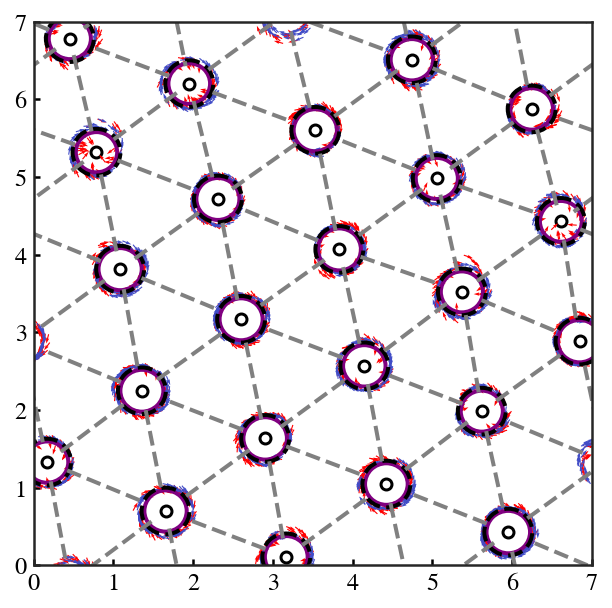
\includegraphics[width=0.49\textwidth]{./figs/latticeConstant.png}
    \caption{
        Snapshots of system at $t=80$ with $N=1000$, $K=10.5$, $d_0=1.07$, $\alpha =0.6\pi$, $\omega _{\min}=0$, and $\Delta \omega =1$.
    }
\end{figure}

\newpage

\begin{figure}[H]
    \centering
    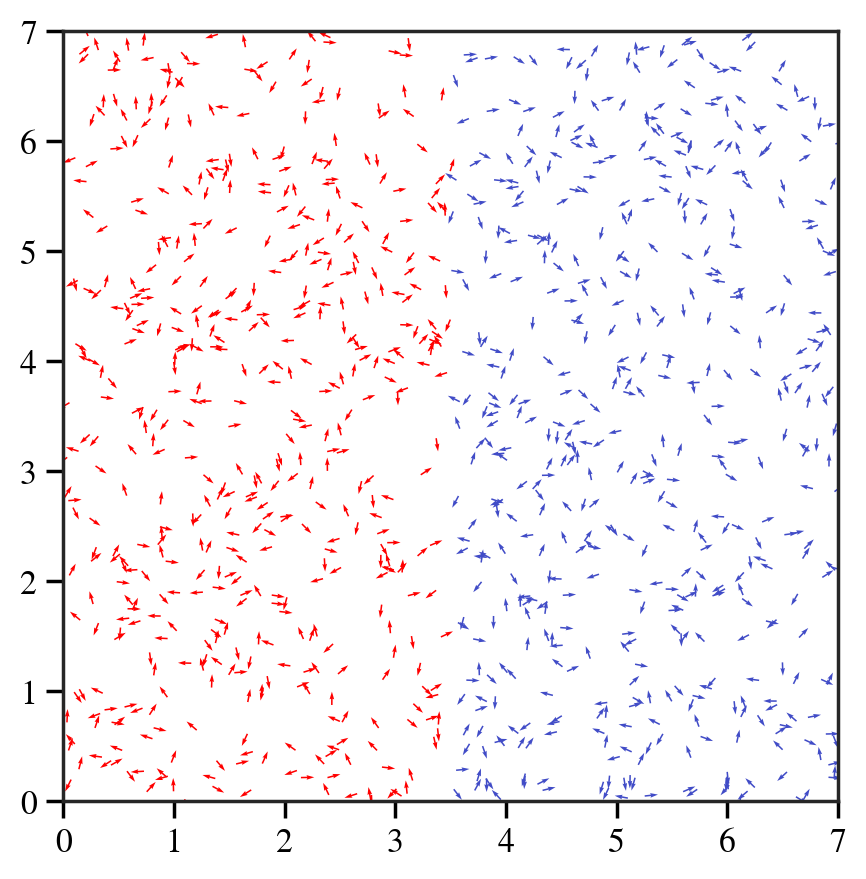
\includegraphics[width=0.4\textwidth]{./figs/halfSide.png}
    \caption{
        Initial conditions of half on each side.
    }
\end{figure}

\begin{figure}[H]
    \centering
    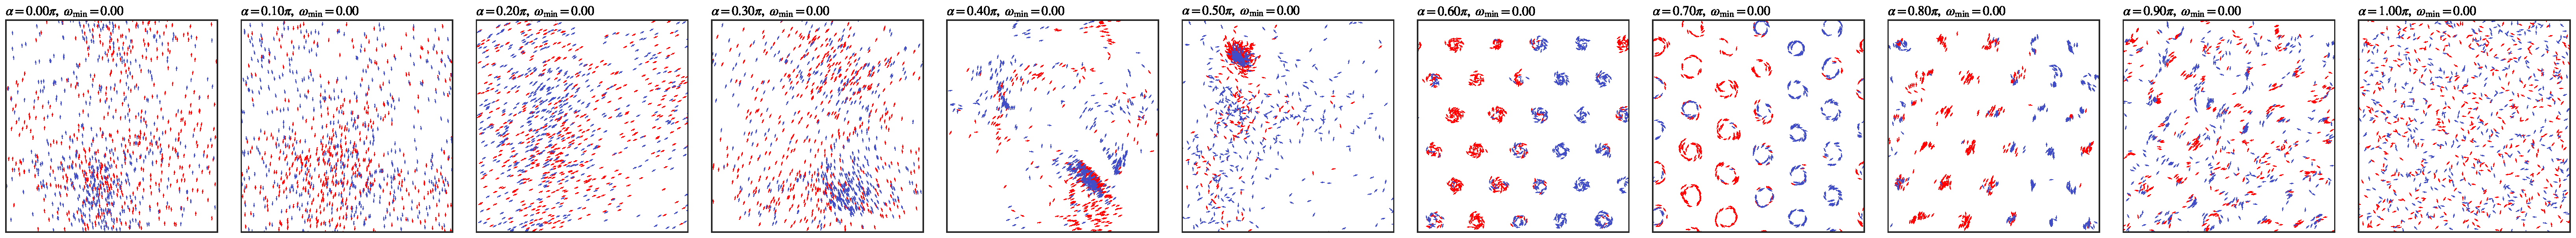
\includegraphics[width=\textwidth]{./figs/HalfInitPhaseLagPatternFormation_a0.00_Do1_aN1000_distuniform.pdf}
    \caption{
        \label{fig:half}
        Snapshot of the system at $t=80$ with $N=1000$, $K=20$, $\omega _{\min}=0$, $\Delta \omega=1$ and initial conditions of half on each side.
    }
\end{figure}

\begin{figure}[H]
    \centering
    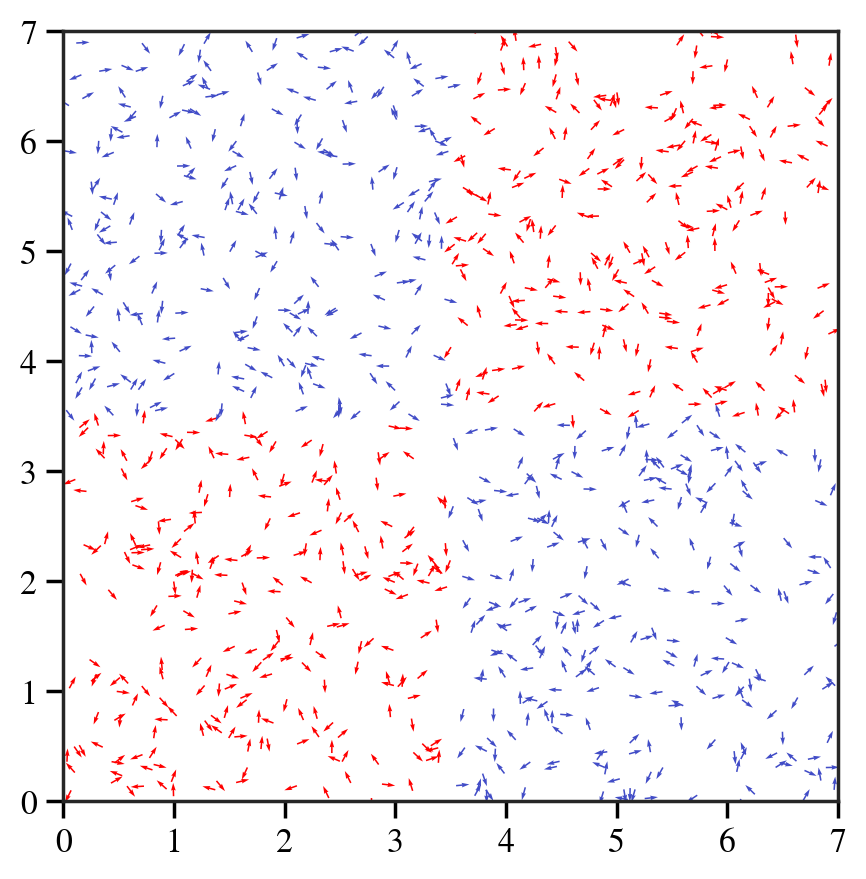
\includegraphics[width=0.4\textwidth]{./figs/chess.png}
    \caption{
        Initial conditions of chessboard pattern.
    }
\end{figure}

\begin{figure}[H]
    \centering
    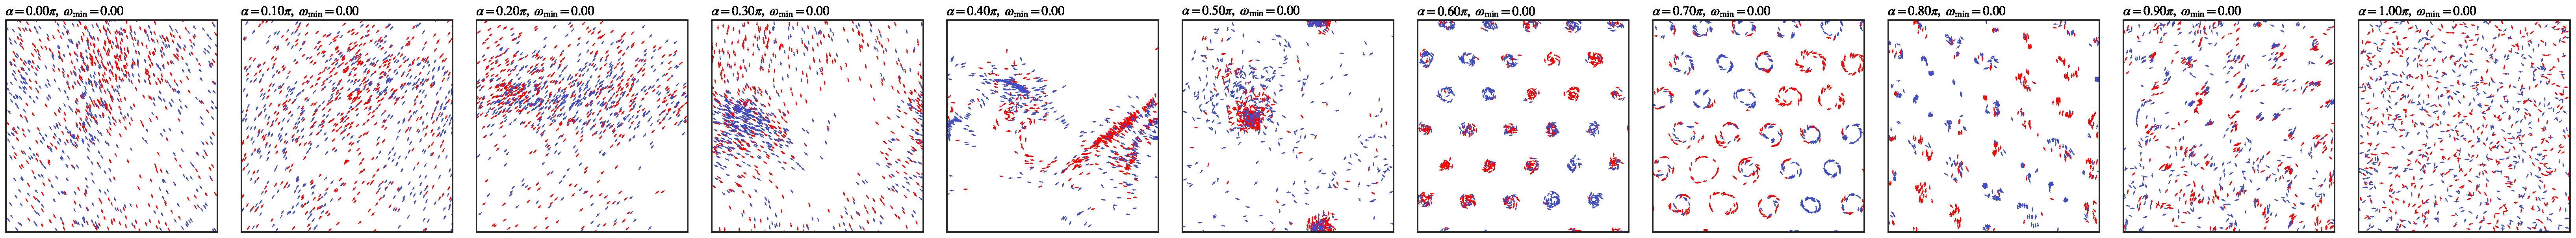
\includegraphics[width=\textwidth]{./figs/ChessboardPhaseLagPatternFormation_a0.00_Do1_aN1000_distuniform.pdf}
    \caption{
        \label{fig:chess}
        Snapshot of the system at $t=80$ with $N=1000$, $K=20$, $\omega _{\min}=0$, $\Delta \omega=1$ and initial conditions of chessboard pattern.
    }
\end{figure}

\begin{figure}[H]
    \centering
    \includegraphics[width=0.75\textwidth]{./figs/snapshot0.6pi.pdf}
    \caption{
        \label{fig:snapshot0.6pi}
        Snapshots of achiral system ($\omega _{\min}=0$ and $\Delta \omega=0$) at different coupling strengths $K$ and radius $d_0$ for $\alpha = 0.6\pi$. 固定阻锉为$0.6\pi$,不同的耦合强度$K$和半径$d_0$下的非手性粒子系统快照。粒子颜色根据其瞬时相位$\theta_i$着色。随着两个耦合参数的增加,粒子在空间中逐渐形成三角晶格结构且尺寸和彼此距离不断增加。
    }
\end{figure}

% \begin{figure}[H]
%     \centering
%     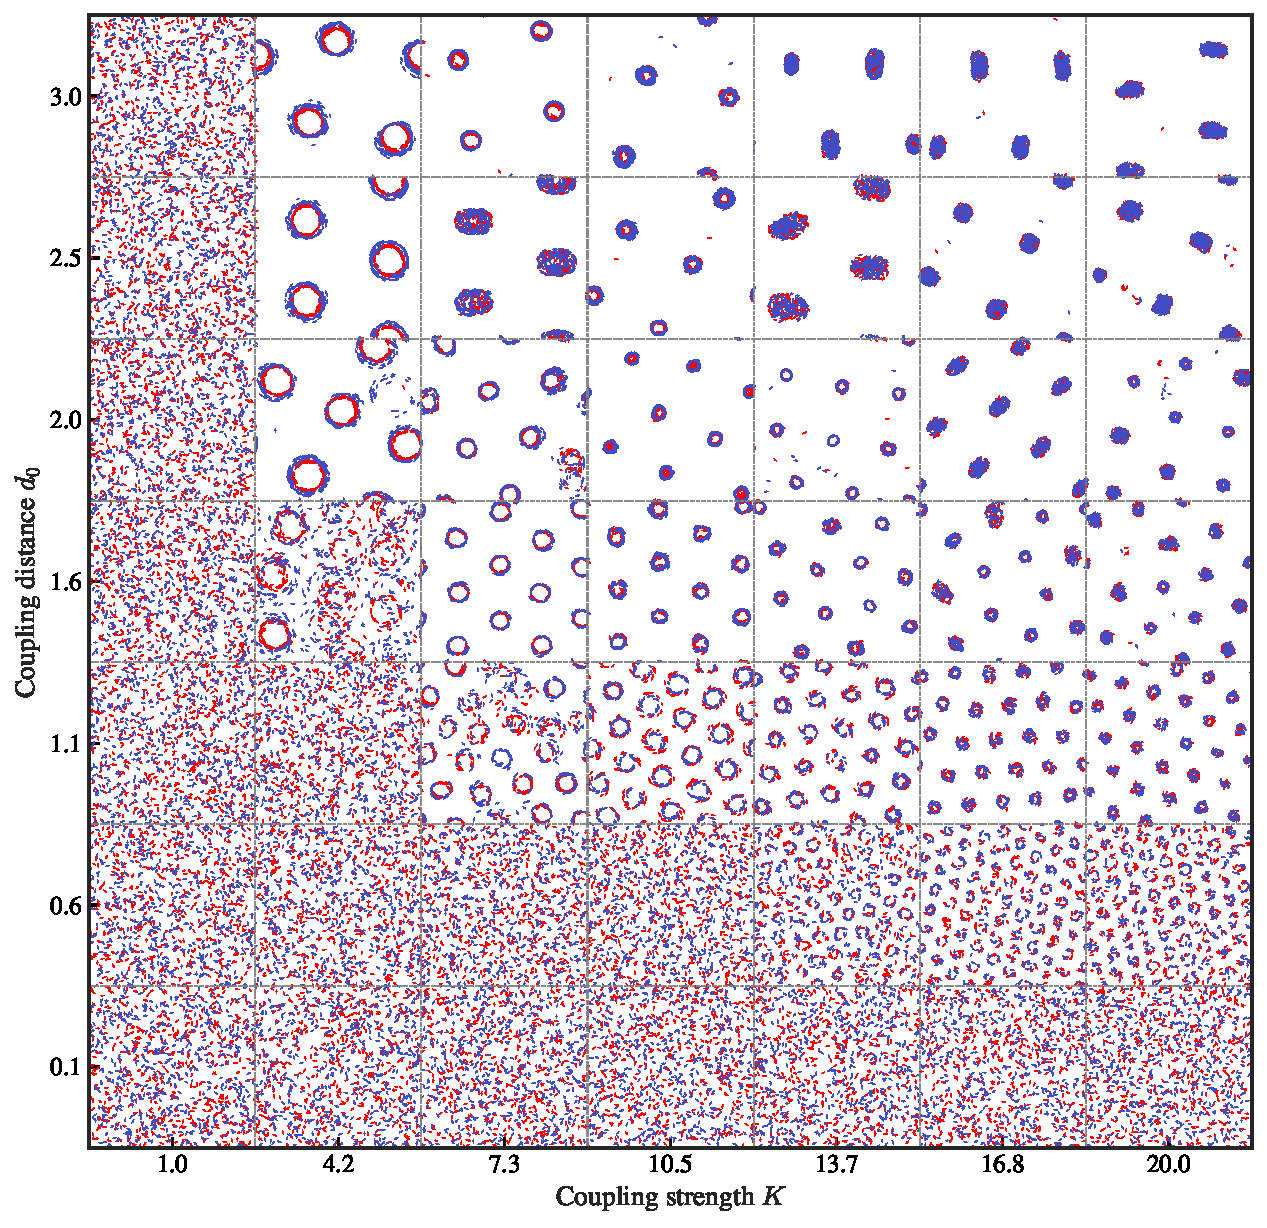
\includegraphics[width=0.75\textwidth]{./figs/PhaseLagPatternFormation_varying_strengthK_and_distanceD0_freq_a1.88_Do1_aN1000.pdf}
%     \caption{
%         \label{fig:snapshot0.6pi_chiral}
%         Snapshots of system at different coupling strengths $K$ and radius $d_0$ with $N=1000$, $K=20$, $\alpha =0.6\pi$, $\omega _{\min}=0$, and $\Delta \omega =1$. 固定阻锉为$0.6\pi$,不同的耦合强度$K$和半径$d_0$下的手性粒子系统快照。粒子颜色根据其瞬时相位$\theta_i$着色。随着两个耦合参数的增加,粒子在空间中逐渐形成三角晶格结构且尺寸和彼此距离不断增加。
%     }
% \end{figure}

% \begin{figure}[H]
%     \centering
%     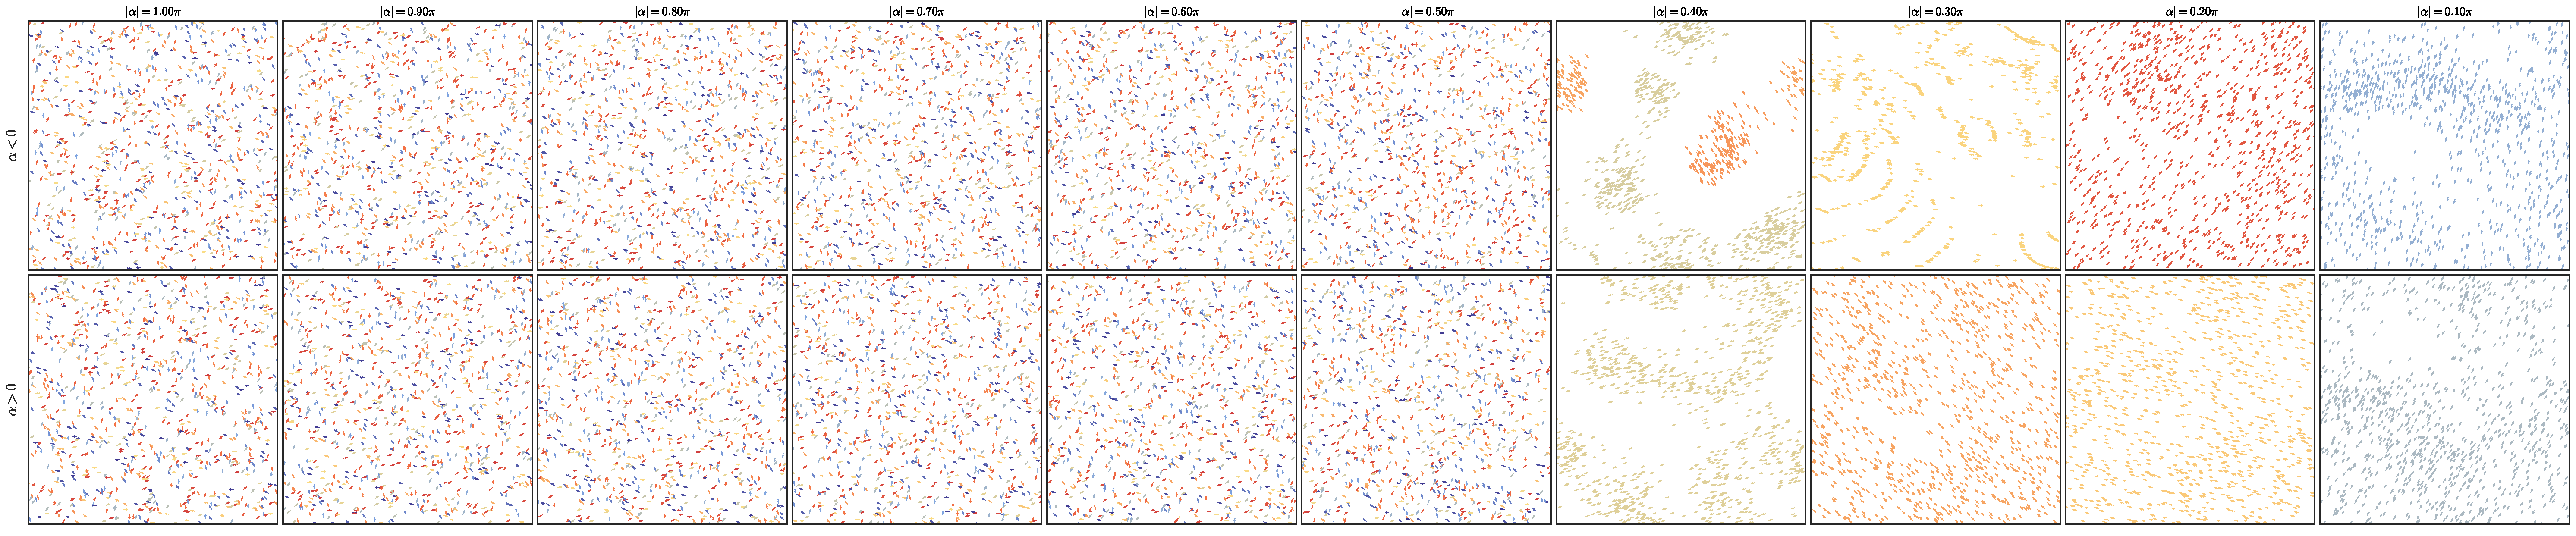
\includegraphics[width=\textwidth]{./figs/noncounter_snapshot.pdf}
%     \caption{
%         Snapshot of the system without counter term $-\sin\alpha$ at $t=80$ with $N=1000$, $K=20$, $\omega _{\min}=0.1$ and $\Delta \omega=1$. The particles are colored according to their instantaneous phase $\theta_i$. There is no triangular lattice structure, and the particles are randomly distributed in space.
%         系统终态的快照,粒子颜色根据其瞬时相位$\theta_i$着色。空间排列没有三角晶格结构,粒子在空间中随机分布。
%     }
%     \label{fig:noncounter_shotsnaps}
% \end{figure}

% \begin{figure}[H]  % 如果希望把图片放在当前段落中,可以使用[H]选项
%     \centering
%     \subcaptionbox{Snapshot}[0.49\linewidth]{
%       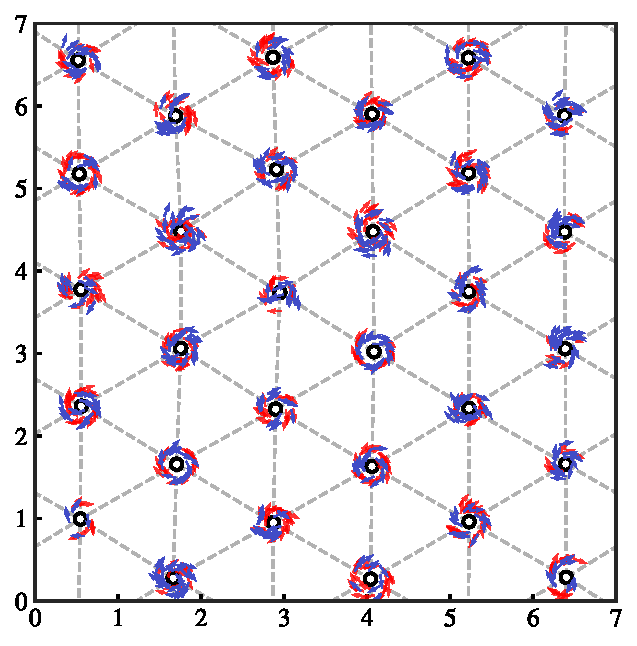
\includegraphics[width=\linewidth]{figs/snapshot.pdf}
%     }
%     \hfill
%     \subcaptionbox{
%         Statistics of cells
%     }[0.49\linewidth]{
%       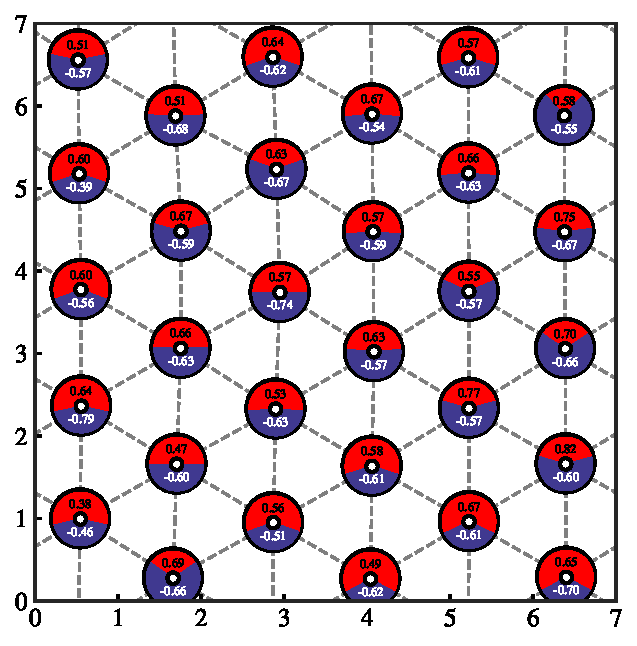
\includegraphics[width=\linewidth]{figs/statistics.pdf}
%     }
%     \caption{
%         Snapshot and statistics of cells of system at $t=80$ with $N=1000$, $K=20$, $\alpha =0.6\pi$, $\omega _{\min}=0.1$, and $\Delta \omega =1$. In \textbf{(b)}, the pie chart shows the proportion of two chiralities in the cell, and the black, white text indicates the mean natural frequency of positive, negative chiral particles in the cell, respectively.
%         系统终态的快照和晶格统计。快照中,粒子晶格呈现三角形晶格结构。饼图显示了正负两种粒子在晶格中的比例,黑色和白色文本分别表示正负粒子的平均自然频率。
%     }
% \end{figure}

% 陆羿辰:从统计结果中看不出临近晶格之间的规律,似乎和粒子数目以及粒子的自然频率无关。

% \begin{figure}[H]  % 如果希望把图片放在当前段落中,可以使用[H]选项
%     \centering
%     \subcaptionbox{
%         Colors represent the mean natural frequency
%     }[0.49\linewidth]{
%       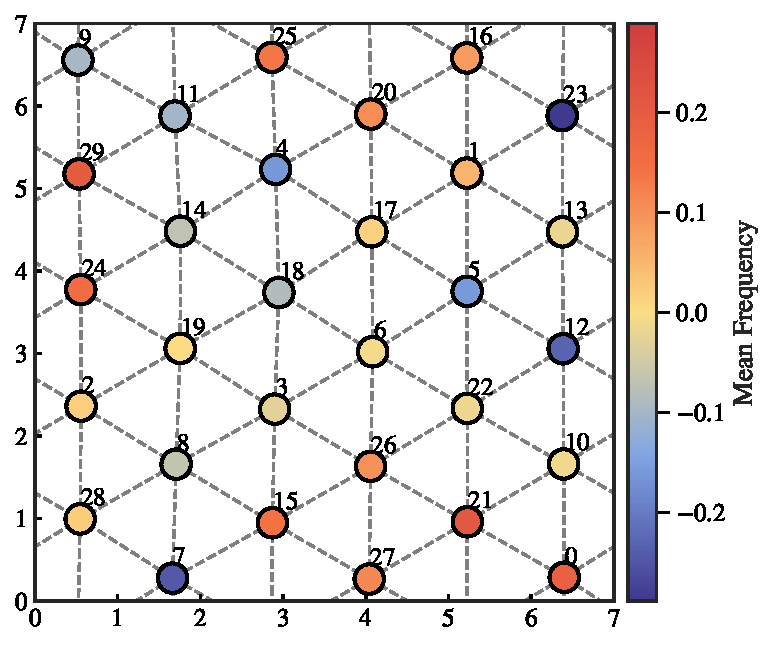
\includegraphics[width=\linewidth]{figs/mean_freq.pdf}
%     }
%     \hfill
%     \subcaptionbox{
%         Colors represent the mean effective frequency
%     }[0.49\linewidth]{
%       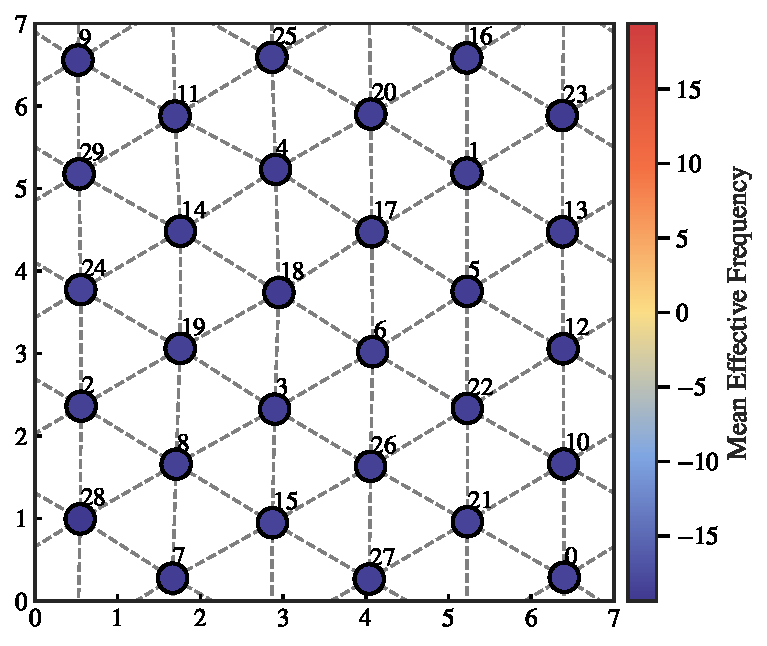
\includegraphics[width=\linewidth]{figs/mean_eff_freq.pdf}
%     }
%     \caption{
%         \label{fig:mean_freq}
%         The mean natural frequency and effective frequency of particles in each cell. The effective frequency is defined as the average instantaneous phase velocity of particles in the cell.
%         \textbf{(a)} shows the mean natural frequency of particles in each cell, while \textbf{(b)} shows the mean effective frequency of particles in each cell.
%         每个晶格中粒子的平均自然频率和有效频率。有效频率定义为晶格中粒子终态瞬时相速度的平均值。\textbf{(a)}显示了每个晶格中粒子的平均自然频率,而\textbf{(b)}显示了每个晶格中粒子的平均有效频率。
%     }
% \end{figure}

\begin{figure}[H]
    \centering
    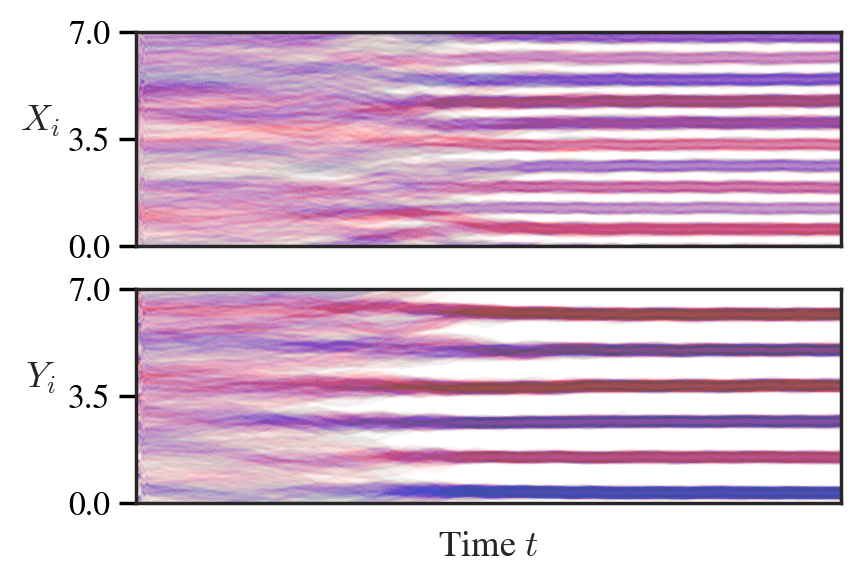
\includegraphics[width=0.6\textwidth]{./figs/Center Scatter.png}
    \caption{
       \label{fig:Center Scatter}
       瞬时旋转中心随时间变化的散点图。其中$N=1000$, $K=20$, $\alpha =0.6\pi$,  $\omega _{\min}=0.1$。随时间演化,粒子晶格大体呈现红蓝交错分布的趋势。
    }
\end{figure}

陆羿辰:从旋转中心的散点图确实能看出一些红蓝交替出现的现象,原因暂时不明(也可能和画散点图时图层的排序有关,可以尝试改变一下图层的顺序)

陆羿辰:调整完图层之后色调发生了改变,目前猜测应该不是类似棋盘格的分布

\section{Phase Diagram and Mechanism}

\subsection{Phase Diagram}

The phase diagram of the system is constructed by varying the key parameters, including the coupling strength $K$, the radius $d_0$. The resulting patterns are classified into ordered and lattice states. 

The order parameter $\sigma _{\rho}\left( t \right)$ is defined as the standard deviation of the density, which quantifies the degree of spatial ordering in the system.
\begin{equation}
    \sigma _{\rho}\left( t \right) =\sqrt{\frac{1}{L^2}\int{\left[ \rho \left( \mathbf{r},t \right) -\left< \rho \left( \mathbf{r},t \right) \right> \right] ^2\mathrm{d}\mathbf{r}}}\;,
\end{equation}
where $\rho \left( \mathbf{r},t \right) =\int_0^{2\pi}{f\left( \mathbf{r},\theta ,t \right) \mathrm{d}\theta}$ is the density of particles at position $\mathbf{r}$ and time $t$, and $\left< \rho \left( \mathbf{r},t \right) \right> =\frac{1}{L^2}\int{\rho \left( \mathbf{r},t \right) \mathrm{d}\mathbf{r}}$ is the average density over the system. 
% The boundaries between these phases are determined by analyzing the stability of the system and the behavior of the order parameter.
\begin{figure}[H]
    \centering
    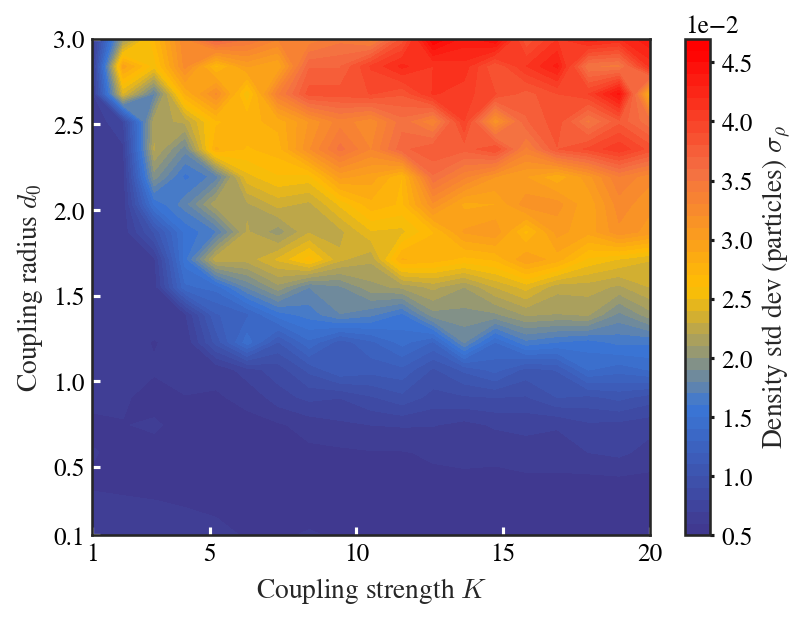
\includegraphics[width=0.6\textwidth]{./figs/orderParameter_varying_strengthK_and_distanceD0.png}
    \caption{
        \label{fig:orderParameter_varying_strengthK_and_distanceD0}
        The order parameter $\sigma _{\rho}\left( t \right)$ as a function of coupling strength $K$ and radius $d_0$. The color indicates the value of the order parameter, with red representing high cohesiveness and blue representing low cohesiveness. 
    }
\end{figure}

\subsection{Hydrodynamics}

Here, we develop a continuum theory for the self-propelled particles with phase frustration, following the approach in \cite{PhysRevLett.119.058002,PhysRevResearch.1.023026}. We start with the Eqs.~(\ref{eq:totalDynamicsMeanField}) but replace the finite range alignment interaction by a pseudopotential ('$\delta$'-interaction), which is justified if the interaction is short ranged enough, such that the shape of the associated interaction potential is irrelevant to the many particle dynamics. Additionally, for simplicity of analysis, we consider achiral systems ($\omega _{i}=0$). T
he \begin{subequations}
    \begin{align}
        \dot{\mathbf{r}}_i&=v\mathbf{p}\left( \theta _i \right) \;,\\
        \dot{\theta}_i&=\frac{K}{\left| A_i \right|}\sum_{j=1}^{N}{\delta \left( \mathbf{r}_j-\mathbf{r}_i \right) \left[ \sin \left( \theta _j-\theta _i+\alpha \right) -\sin \alpha \right]} \;.
    \end{align}
\end{subequations}

In the thermodynamic limit $N\rightarrow \infty$, the agent-based model gives rise to the following continuum form:
\begin{equation}
    \frac{\partial}{\partial t}f\left( \mathbf{r},\theta ,t \right) = -\nabla \cdot \left( f\mathbf{v}_{\mathbf{r}} \right) -\frac{\partial}{\partial \theta}\left( fv_{\theta} \right)\;,
    \label{eq:continuum}
\end{equation}
where $f\left( \mathbf{r},\theta ,t \right)$ is the probability density of particles at position $\mathbf{r}$ and orientation $\theta$ at time $t$, and $\mathbf{v}_{\mathbf{r}}$ and $v_{\theta}$ are the velocity fields in the position and orientation space, respectively. The velocity fields are given by
\begin{subequations}
    \begin{align}
        \mathbf{v}_{\mathbf{r}}\left( \mathbf{r},\theta ,t \right) &=v\mathbf{p}\left( \theta \right)\\
        v_{\theta}\left( \mathbf{r},\theta ,t \right) &=-\sin \alpha +K\int{\mathrm{d}\theta ^{\prime}f\left( \mathbf{r},\theta ^{\prime},t \right) \sin \left( \theta ^{\prime}-\theta +\alpha \right)}\;.
    \end{align}
    \label{eq:velocityFields}
\end{subequations}
By substituting Eqs.~\eqref{eq:velocityFields} into Eq.~\eqref{eq:continuum}, we obtain 

\subsection{Abstract phase oscillator model}
Let us consider a decoupled phase-oscillator system 
\begin{equation}
    \dot{\theta}_i=\omega _i-K\sin \alpha +\frac{K}{N}\sum_{j=1}^N{\sin \left( \theta _j-\theta _i+\alpha \right)}\;.
    \label{eq:decoupledPhaseModel}
\end{equation}

To quantify the phase coherence of the system, it is convenient to define the generalized complex-valued order parameters, i.e.,
\begin{equation}
    \label{eq:orderParameter}
    Z\left( t \right) =R\left( t \right) \text{e}^{\text{i}\psi\left( t \right)}=\frac{1}{N}\sum_{j=1}^N{\text{e}^{\text{i}\theta _{j}\left( t \right)}}\;,
\end{equation}
where $n=1,2,\dots, N$, and $r\left( t \right)$, $\psi \left( t \right)$ are the amplitudes and arguments of the order parameter.
Our starting point is to analyze the critical point for the coherence of the order parameter.
In the thermodynamic limit $N\to \infty$, the state of the system in Eq.~(\ref{eq:decoupledPhaseModel}) can be characterized by the single-oscillator distribution $\rho\left( \theta ,\omega, t \right)$, which satisfies the continuity equation
\begin{equation}
    \frac{\partial \rho}{\partial t}+\frac{\partial \left( \rho v \right)}{\partial \theta}=0\;,
    \label{eq:continuityEquation}
\end{equation}
where $\rho \left( \theta ,\omega ,t \right)$ accounts for the fraction of oscillators with phase $\theta$ lying in the interval $\left( \theta ,\theta +\mathrm{d}\theta \right)$ at fixed frequency $\omega$ and time $t$, it satisfies the normalization condition
\begin{equation}
    \label{eq:normalization}
    \int_{0}^{2\pi}{\rho \left( \theta ,\omega ,t \right) \text{d}\theta} =1\;.
\end{equation}
Here, $v\left( \theta ,\omega ,t \right)$ is the velocity field, given by
\begin{equation}
    \begin{aligned}
        v\left( \theta ,\omega ,t \right) =&K\int_{-\infty}^{+\infty}{\int_0^{2\pi}{\sin \left( \theta ^{\prime}-\theta +\alpha \right) \rho \mathrm{d}\theta ^{\prime}\mathrm{d}\omega ^{\prime}}}\\
        &+\omega -K\sin \alpha \;.
    \end{aligned} 
\end{equation}
Correspondingly, the order parameter defined in Eq.~(\ref{eq:orderParameter}) in the thermodynamic limit reads
\begin{equation}
    Z\left( t \right) =\int_{-\infty}^{+\infty}{g\left(\omega\right)\mathrm{d}\omega \int_0^{2\pi}{\mathrm{e}^{\mathrm{i}\theta}\rho \left( \theta ,\omega ,t \right) \mathrm{d}\theta }} \;,
    \label{eq:orderParameterContinuum}
\end{equation}
then $v\left( \theta ,\omega ,t \right)$ simplifies to
\begin{equation}
    v\left( \theta ,\omega ,t \right) =\omega -K\sin \alpha +\mathrm{Im}\left[ H\left( t \right) \mathrm{e}^{-\mathrm{i}\theta} \right] \;,
    \label{eq:velocityField}
\end{equation}
with the mean-field being
\begin{equation}
    H\left( t \right) =KZ\left( t \right) \mathrm{e}^{\mathrm{i}\alpha} \;.
\end{equation}

Since the distribution $\rho \left( \theta ,\omega ,t \right)$ is $2\pi$-periodic in $\theta$, we can expand it in Fourier series as
\begin{equation}
    \rho \left( \theta ,\omega ,t \right) =\frac{1}{2\pi}\sum_{n=-\infty}^{+\infty}{a _n\left( \omega ,t \right) \mathrm{e}^{\mathrm{i}n\theta}}\;,
    \label{eq:rhoFourier}
\end{equation}
where $a _n\left( \omega ,t \right)$ is the $n$-th Fourier coefficient. In particular, we have $a _0\left( \omega ,t \right) \equiv 1$ owing to the normalization condition in Eq.~(\ref{eq:normalization}) and $a _{-n}\left( \omega ,t \right) =a _n^{*}\left( \omega ,t \right)$, where $*$ denotes the complex conjugate.

According to the Ott-Antonsen ansatz \cite{10.1063/1.2930766,10.1063/1.3136851}, it states that the $n$-th Fourier coefficient $a_n\left(\omega, t\right)$ can be expressed in terms of the first-order coefficient, i.e., $a_n\left(\omega, t\right) = a^{n}\left(\omega, t\right)$. In this regard, the evolution of $\rho\left(\theta, \omega, t\right)$ degenerates to an invariant manifold, which is
\begin{equation}
    \dot{a}\left( t \right) =\mathrm{i}\left( K\sin \alpha -\omega \right) a\left( t \right) +\frac{1}{2}\left[ H^{*}\left( t \right) -H\left( t \right) a^2\left( t \right) \right] \;.
    \label{eq:OttAntonsen}
\end{equation}
Consequently, Eq.~(\ref{eq:OttAntonsen}) is closed by the definition of the order parameter in Eq.~(\ref{eq:orderParameterContinuum}), where
\begin{equation}
    \begin{aligned}
        Z\left( t \right) &=\int_{-\infty}^{+\infty}{g\left( \omega \right) a_{-1}\left( \omega ,t \right) \mathrm{d}\omega} \;,\\
        &=\int_{-\infty}^{+\infty}{g\left( \omega \right) a^{*}\left( \omega ,t \right) \mathrm{d}\omega} \;.\\
    \end{aligned}
    \label{eq:orderParameterOttAntonsen}
\end{equation}

We stress that Eq.~(\ref{eq:OttAntonsen}) is still infinite dimensional
because of the distributed natural frequencies. Thus, we may make a specific choice for the frequency distribution to get around this difficulty, e.g. a Lorentzian distribution $g\left(\omega\right)=\varDelta / [ \pi\left(\omega-\mu\right)^2+\varDelta ^2 ]$ with $\varDelta $ being the width of the distribution and $\mu$ being the mean frequency.
In this setting, the order parameters defined in Eq.~(\ref{eq:orderParameterOttAntonsen}) can be calculated by using Cauchy's residue theorem with analytical continuation of $a\left(\omega, t\right)$ into the lower half complex plane, which leads to
\begin{equation}
    Z(t)=a^{*}\left(\mu-\mathrm{i}\varDelta, t\right) \;.
\end{equation}
As a result, the low-dimensional evolution of the order parameter can be obtained by replacing $\omega$ with $\mu-\mathrm{i}\varDelta$ and by taking into account the complex conjugate, which reads
\begin{equation}
    \dot{Z}=-\Delta Z+\mathrm{i}Z\left( \mu -K\sin \alpha \right) +\frac{1}{2}\left[ KZ\mathrm{e}^{\mathrm{i}\alpha}-KZ^*Z^2\mathrm{e}^{-\mathrm{i}\alpha} \right] \;.
    \label{eq:orderParameterEvolution}
\end{equation}
Rewrite above equation using polar coordinates $Z\left( t \right) =R\left( t \right) \mathrm{e}^{\mathrm{i}\psi \left( t \right)}$, we have
\begin{subequations}
    \begin{align}
        \dot{R}&=\frac{R}{2}\left( K-2\varDelta -KR^2 \right) \cos \alpha \;, \label{eq:dotAmplitudeR}\\
        \dot{\psi}&=\mu +\frac{K}{2}\left( R^2-1 \right) \sin \alpha \label{detPsi}\;.
    \end{align}
\end{subequations}
Obviously, the amplitude $R\left( t \right)$ is decoupled from the mean phase $\psi\left( t \right)$ and Eq.~(\ref{eq:dotAmplitudeR}) have a critical coupling strength $K_c=2\varDelta$ and a pair of critical phase frustration $\left|\alpha_c\right| = \pi/2$.
Let us first consider the simplest case of $ \varDelta =0, \mu=0$, which corresponds to the case of achiral particles. In this case, when $\left|\alpha_c\right| > \pi/2$, the system bifurcates to $R=0$, which corresponds to the incoherent state in phase oscillators and lattice state in self-propelled particles, while for $\left|\alpha_c\right| < \pi/2$, the system has a unique stable fixed point at $R=1$, which corresponds to the coherent state and swarming state, respectively.

For the incoherent state, the system is totally disordered with the phases distributed uniformly around the unit circle, i.e., $\rho\left(\theta, \omega, t\right) = g(\omega)/2\pi$, which implies that the phase velocity of each oscillator/particle becomes
\begin{equation}
    \dot{\theta}_i=\omega_i-K\sin \alpha \;.
\end{equation}
Correspondingly, the rotational radii of $i$-th particle is
\begin{equation}
    r_i=\frac{v}{\dot{\theta}_i}=\frac{v}{\omega _i-K\sin \alpha}\;.
\end{equation}


\bibliography{ref}

\end{document}